\section{Time shift response functions}\label{sec:time_shift}

We used the definition of the response function from \cite{Wang_2016_cross} that
is showed in Equation \ref{eq:Wang_2016}. To see the impact of the time shift I
analyzed the TAQ data in the year 2008. I used different time shifts in the
response function

\begin{equation}\label{eq:time_shift_general}
    R_{ij}^{s, escale}\left(\tau\right)=\left\langle r_{i}
    \left(t-t_{s},\tau\right) \cdot\varepsilon^{scale}_{j}
    \left(t\right)\right\rangle _{scale}
\end{equation}

Making $\tau$ constant, and varying $t_{s}$ I obtained values for self- and
cross-responses. CORREGIR As $t_{shift}$ is related with the response, the shift is in
seconds for both scales.

In Sect. \ref{subsec:time_shift_trade} we analyze the influence of the time
shift between the trade signs and returns in trade time scale and in Sect.
\ref{subsec:time_shift_physical} we analyze the influence of the time shift
between the trade signs and returns in physical time scale.

\subsection{Trade time scale shift response functions}
\label{subsec:time_shift_trade}

In Fig. \ref{fig:shift_trade_scale}, for fixed $\tau$ values, there is a peak
in a position related to $\tau$.

In the trade time scale, I tested the response function for different shifted
times (Fig. \ref{fig:shift_responses_trade_scale}). The one second shift curve
is the control curve. From small $\tau$ values to a $\tau_{max}$ value the
response grows. Then it starts to decay, but not under the original value of
$t_{shift} = 1$.

\begin{figure*}[htbp]
    \centering
    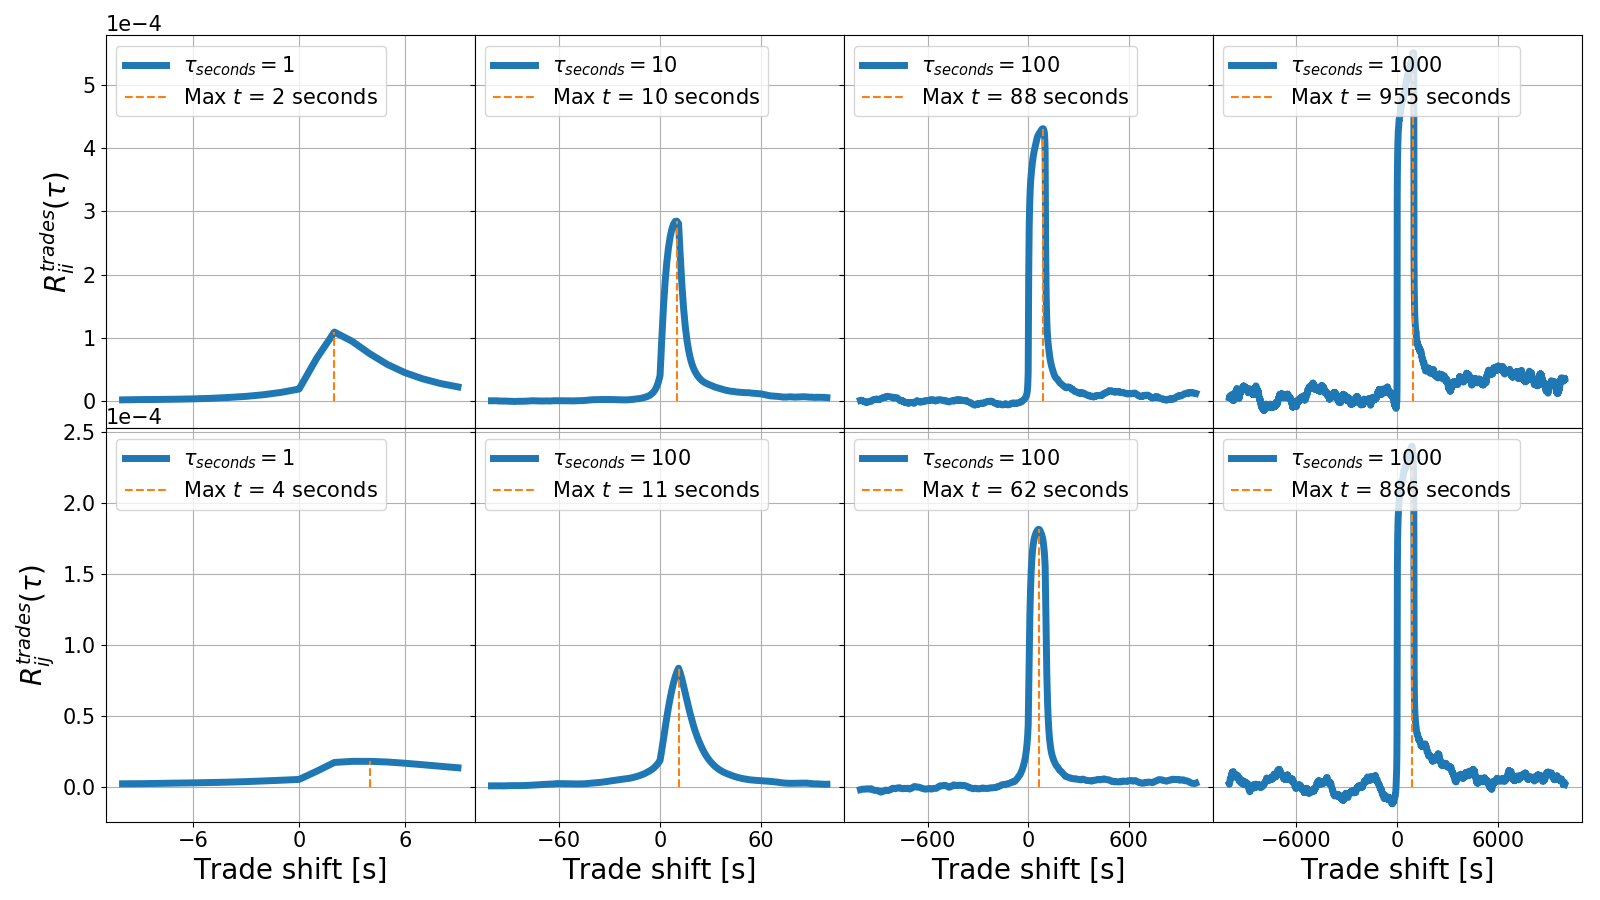
\includegraphics[width=\textwidth]{figures/04_shift_trade.png}
    \caption{Self-response functions $R_{ii}^{trades}\left(\tau\right)$
             excluding $\varepsilon^{trades}_{i}\left(t\right) = 0$ in 2008
             versus shift for the Goldman Sachs Group stock (top) and
             cross-response functions $R_{ij}^{trades}\left(\tau\right)$
             excluding $\varepsilon^{trades}_{j}\left(t\right) = 0$ in 2008
             versus shift for the Goldman Sachs Group-JPMorgan Chase stocks
             (bottom).}
    \label{fig:shift_trade_scale}
\end{figure*}

\begin{figure*}[htbp]
    \centering
    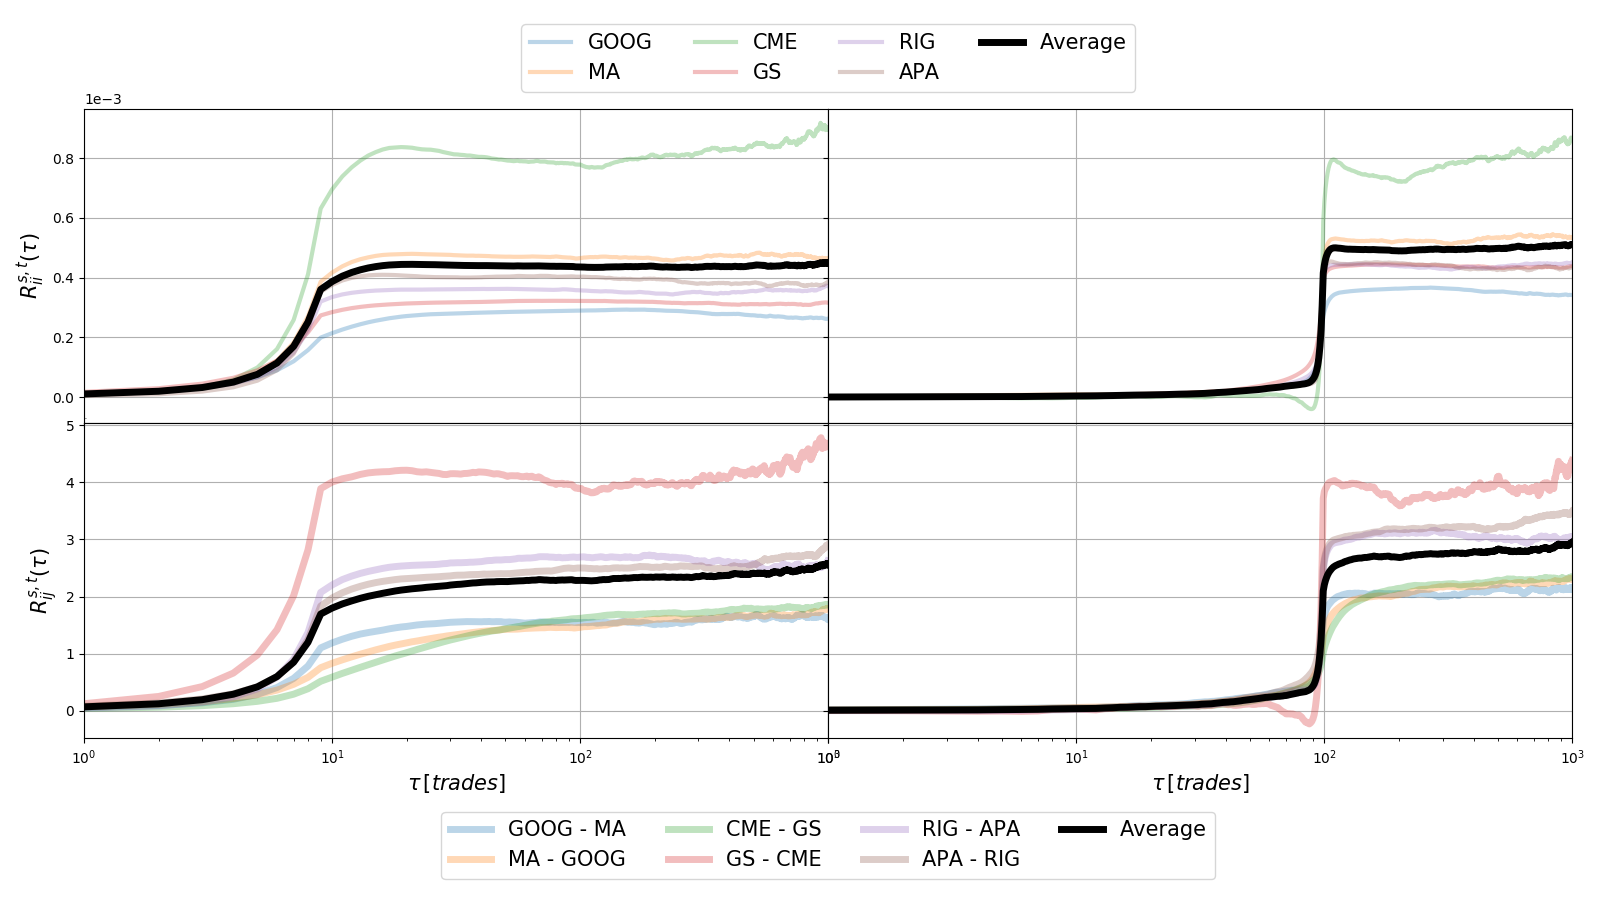
\includegraphics[width=\textwidth]{figures/04_shift_responses_trade.png}
    \caption{Self- and cross-response functions
             $R^{trades}_{ij}\left(\tau\right)$ excluding
             $\varepsilon^{trades}_{j}\left(t\right) = 0$ in 2008 versus time
             lag $\tau$ on a logarithmic scale for different shifts.
             Self-responses for the Goldman Sachs Group stock in trade time
             scale (left), and cross-response of Goldman Sachs Group-JPMorgan
             Chase stocks in trade time scale (right).}
    \label{fig:shift_responses_trade_scale}
\end{figure*}

\subsection{Physical time scale shift response functions}
\label{subsec:time_shift_physical}

For every $\tau$ value, there is a peak. The peak grows fast and decay slowly
for $\tau < 10$, and grows and decays fast for large $\tau$. The response
signal usually starts to grow on zero or a little bit earlier and grows to
around $\tau$.

\begin{figure*}[htbp]
    \centering
    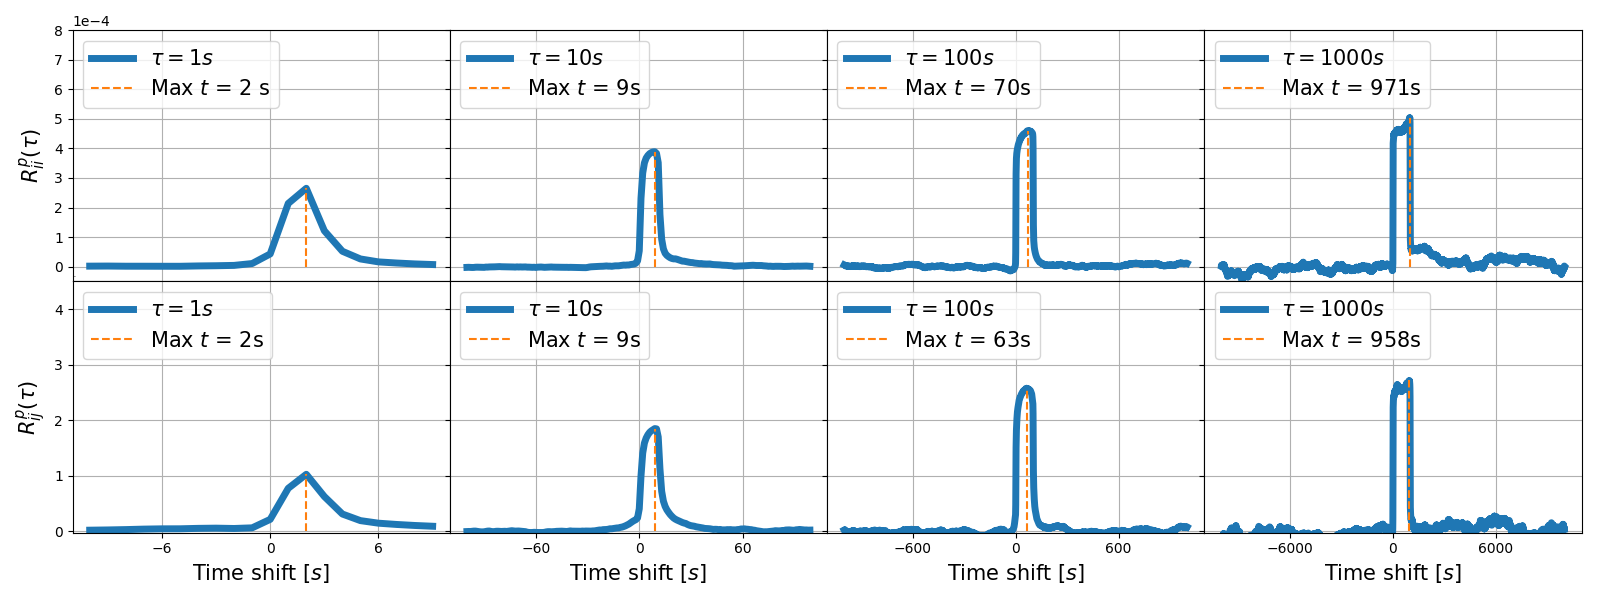
\includegraphics[width=\textwidth]{figures/04_shift_physical.png}
    \caption{Self-response functions $R_{ii}^{seconds}\left(\tau\right)$
             excluding $\varepsilon^{seconds}_{i}\left(t\right) = 0$ in 2008
             versus shift for the Goldman Sachs Group stock (top) and
             cross-response functions $R_{ij}^{seconds}\left(\tau\right)$
             excluding $\varepsilon^{seconds}_{j}\left(t\right) = 0$ in 2008
             versus shift for the Goldman Sachs Group-JPMorgan Chase stocks
             (bottom).}
    \label{fig:shift_physical_scale}
\end{figure*}

I tested the response function for different shifted times (Fig.
\ref{fig:shift_responses_physical_scale}). The one second shift curve is the control curve. From small
$\tau$ values to a $\tau_{max}$ value the response grows. Then it starts to decay, but not under the
original value of $t_{shift} = 1$.

\begin{figure*}[htbp]
    \centering
    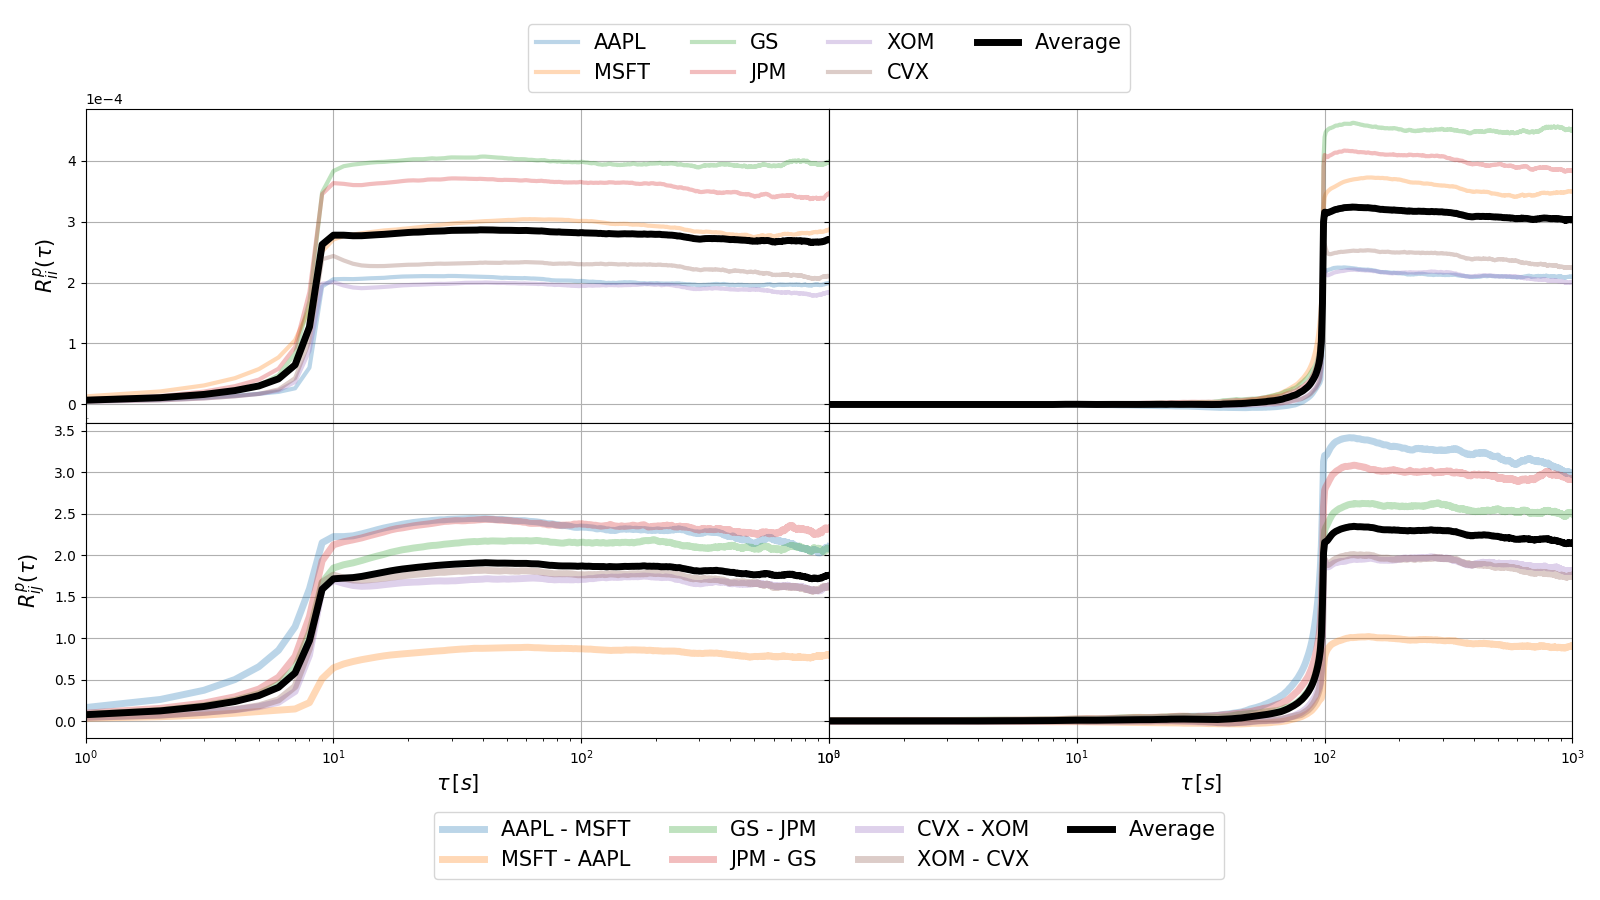
\includegraphics[width=\textwidth]{figures/04_shift_responses_physical.png}
    \caption{Self- and cross-response functions
             $R^{seconds}_{ij}\left(\tau\right)$ excluding
             $\varepsilon^{seconds}_{j}\left(t\right) = 0$ in 2008 versus time
             lag $\tau$ on a logarithmic scale for different shifts.
             Self-responses for the Goldman Sachs Group stock in physical time
             scale (left), and cross-response of Goldman Sachs Group-JPMorgan
             Chase stocks in second time scale (right).}
    \label{fig:shift_responses_physical_scale}
\end{figure*}

My interpretation for the rise of the signal in the different cases, is that there is a zone of the
beginning of the shifted signals where there is not relevant information, which make the response
zero. When the signal reach the one or two event/second shift, the response have again relevant
information, and the response is different to zero.

When the $\tau$ value grows, the averaging value decrease, hence the apparent response is bigger.
This explains that in larger values the signal seems to be large.